\documentclass[conference]{IEEEtran}
\IEEEoverridecommandlockouts

\usepackage[utf8]{inputenc}
\usepackage[portuguese]{babel}
\usepackage{amsmath,amssymb,amsfonts}
\usepackage{graphicx}
\usepackage{textcomp}
\usepackage{xcolor}
\usepackage{float}
\usepackage{xurl}

\def\BibTeX{{\rm B\kern-.05em{\sc i\kern-.025em b}\kern-.08em T\kern-.1667em\lower.7ex\hbox{E}\kern-.125emX}}

\begin{document}

	\title{Aplicação e Análise de Métodos de Regressão}

	\author{\IEEEauthorblockN{Hebert Alan Kubis}
	\IEEEauthorblockA{\textit{Engenharia Mecatrônica} \\
	\textit{Universidade Federal de Santa Catarina (UFSC)}\\
	Centro Tecnológico de Joinville, Brasil}
	}

	\maketitle

	\begin{abstract}

		O presente artigo descreve a avaliação de algoritmos de aprendizado de máquina na previsão de preços de veículos usados. Após um rigoroso pré-processamento (limpeza, remoção de outliers e engenharia de atributos), cinco métodos (K-Neighbors, Ridge, Decision Tree, Random Forest e MLP) foram otimizados via Grid Search. Os resultados mostram que modelos baseados em árvores de decisão e ensembles superaram amplamente os baselines lineares, capturando com precisão as não-linearidades complexas do mercado automotivo.

	\end{abstract}

	\begin{IEEEkeywords}

		Aprendizado de Máquina, Regressão, Previsão de Preços, Engenharia de Atributos, Otimização de Hiperparâmetros.

	\end{IEEEkeywords}

	\section{Introdução}

		O mercado de veículos usados possui precificação volátil, influenciada por quilometragem, especificações e estado de conservação. Abordagens tradicionais de avaliação costumam ser imprecisas. Neste contexto, o Aprendizado de Máquina surge como solução robusta. Este trabalho aplica e compara métodos de regressão em uma base automotiva, buscando a abordagem preditiva mais eficaz para estabelecer um baseline de desempenho sólido.

	\section{Análise da Base de Dados}

		A análise de desempenho de diferentes métodos de regressão iniciou-se pela exploração dos dados fornecidos. A base possui várias características de diversos carros, sendo cada veículo uma instância. O objetivo da inserção desses dados em um modelo é estimar o preço com base em seus atributos.

		A primeira etapa consistiu em excluir da base de treino todas as instâncias nas quais o preço estava ausente. Adicionalmente, procedeu-se com a remoção de outliers, eliminando veículos com preços irreais inferiores a U\$ 1.000, bem como as instâncias que representavam o 1\% dos veículos mais caros da base. Essa abordagem visou mitigar erros de digitação na variável alvo, assumindo que alguns veículos de superluxo também foram removidos no corte superior para estabilizar a matemática dos modelos. Esse filtro resultou na exclusão de aproximadamente 19\% da base de treino inicial. Para reduzir a dimensionalidade e a redundância, a coluna "Faixa\_Preco" foi removida, visto que esta informação já estava contida na variável contínua de preço.

		O pré-processamento de variáveis categóricas transformou atributos como "Adesivos\_personalizados" e "Couro" em valores binários. Em seguida, a técnica de One-Hot Encoding (dummy variables) foi aplicada aos atributos: "Categoria", "Combustível", "Tipo\_cambio", "Tração", "Fabricante" e "Cor", sendo que nesta última realizou-se um agrupamento semântico unindo "Azul ceu" com "Azul" e "Red" com "Vermelho" para reduzir a cardinalidade.

		Outra etapa crucial da engenharia de atributos separou a informação do volume do motor do fato de o carro ser turbo (criando um novo atributo binário). Foram descartadas instâncias com volume de motor igual a zero, visto que a base não compreendia veículos puramente elétricos. O atributo "Portas" foi convertido em uma escala ordinal por ordem de grandeza (0 a 2), sob a premissa de que veículos com mais portas tendem a apresentar dinâmicas de preço distintas.

		Para a variável de quilometragem ("Km"), os dados nulos foram imputados utilizando a mediana dos veículos agrupados pelo mesmo "Ano" de fabricação. Por fim, as funcionalidades de rádio foram separadas nas colunas binárias "AM" e "FM", e a coluna descritiva do "Modelo" do veículo foi excluída devido à sua altíssima cardinalidade (mais de 1.000 modelos distintos), o que geraria excesso de ruído nos algoritmos.

		Após a higienização completa, constatou-se que cerca de 20\% da base original de treino foi excluída, restando 7.772 das 8.685 instâncias iniciais. Ressalta-se que a base de testes foi submetida ao exato mesmo pipeline de tratamento, garantindo o alinhamento de matrizes.

	\section{Métricas de Desempenho}

		Para analisar e comparar a qualidade preditiva de cada modelo, foram adotadas as seguintes métricas estatísticas:

		\begin{itemize}
			\item MAE (Mean Absolute Error): Representa a média do erro absoluto, indicando em quantos dólares, em média, as previsões do modelo divergiram do preço real do veículo no mercado.
			\item RMSE (Root Mean Squared Error): Calcula a raiz quadrada da média dos erros elevados ao quadrado. Por utilizar uma penalidade quadrática, esta métrica é altamente sensível a erros grosseiros (outliers residuais), sendo excelente para verificar se o modelo cometeu equívocos absurdos de precificação.
			\item R² (R-Squared): O Coeficiente de Determinação mede a proporção da variância nos preços que é previsível a partir das variáveis de entrada. Atua como um medidor percentual (0 a 1) do quanto o modelo efetivamente aprendeu sobre o comportamento do mercado.
		\end{itemize}

	\section{Testes e Resultados}

		Para cada modelo foi feita uma busca automatizada de hiperparâmetros (Grid Search) utilizando o Coeficiente de Determinação ($R^2$) como métrica de seleção, visto que ele fornece uma interpretação percentual direta de quão bem o modelo explica a variância dos dados. A otimização definiu as seguintes configurações: \textbf{K-Neighbors} ($n\_neighbors=10$, $weights=\text{'distance'}$, $p=1$), priorizando vizinhos próximos via distância de Manhattan; \textbf{Ridge} ($\alpha=110.0$), aplicando forte regularização L2 para reduzir pesos de variáveis irrelevantes e evitar overfitting; \textbf{Decision Tree} ($max\_depth=15$, $min\_samples\_split=32$, $min\_samples\_leaf=6$), restringindo ramificações isoladas para forçar a generalização; \textbf{Random Forest} ($n\_estimators=180$, $max\_depth=\text{None}$, $min\_samples\_split=2$), criando um conjunto de árvores profundas para capturar padrões não-lineares; e \textbf{MLP}, que manteve a topologia padrão do Scikit-Learn (100 neurônios, ativação ReLU, taxa de aprendizado constante) pois arquiteturas mais profundas sofreram sobreajuste neste volume de dados.

		Deste modo, a tabela a seguir mostra os valore obtidos para as metricas determinadas no trabalho para cada um dos modelos testados:

		\begin{table}[htbp]
			\centering
			\caption{Desempenho dos modelos}
			\resizebox{\linewidth}{!}{
				\begin{tabular}{|l|c|c|c|}
					\hline
					\textbf{Model} & \textbf{MAE} & \textbf{RMSE} & \textbf{R²} \\ \hline
					K-Neighbors & \$ 7085.93 & \$ 10591.17 & 0.4909 \\ \hline 
					Ridge & \$ 8096.72 & \$ 11342.61 & 0.4160 \\ \hline
					Tree & \$ 5619.51 & \$ 8890.14 & 0.6413 \\ \hline
					Forest & \$ 4621.95 & \$ 7506.02 & 0.7443\\ \hline
					MLP & \$ 5796.82 & \$ 8840.99 & 0.6452 \\ \hline
				\end{tabular}
			}
			\label{tab:metricas}
		\end{table}

		\begin{figure}[htbp]
			\centering
			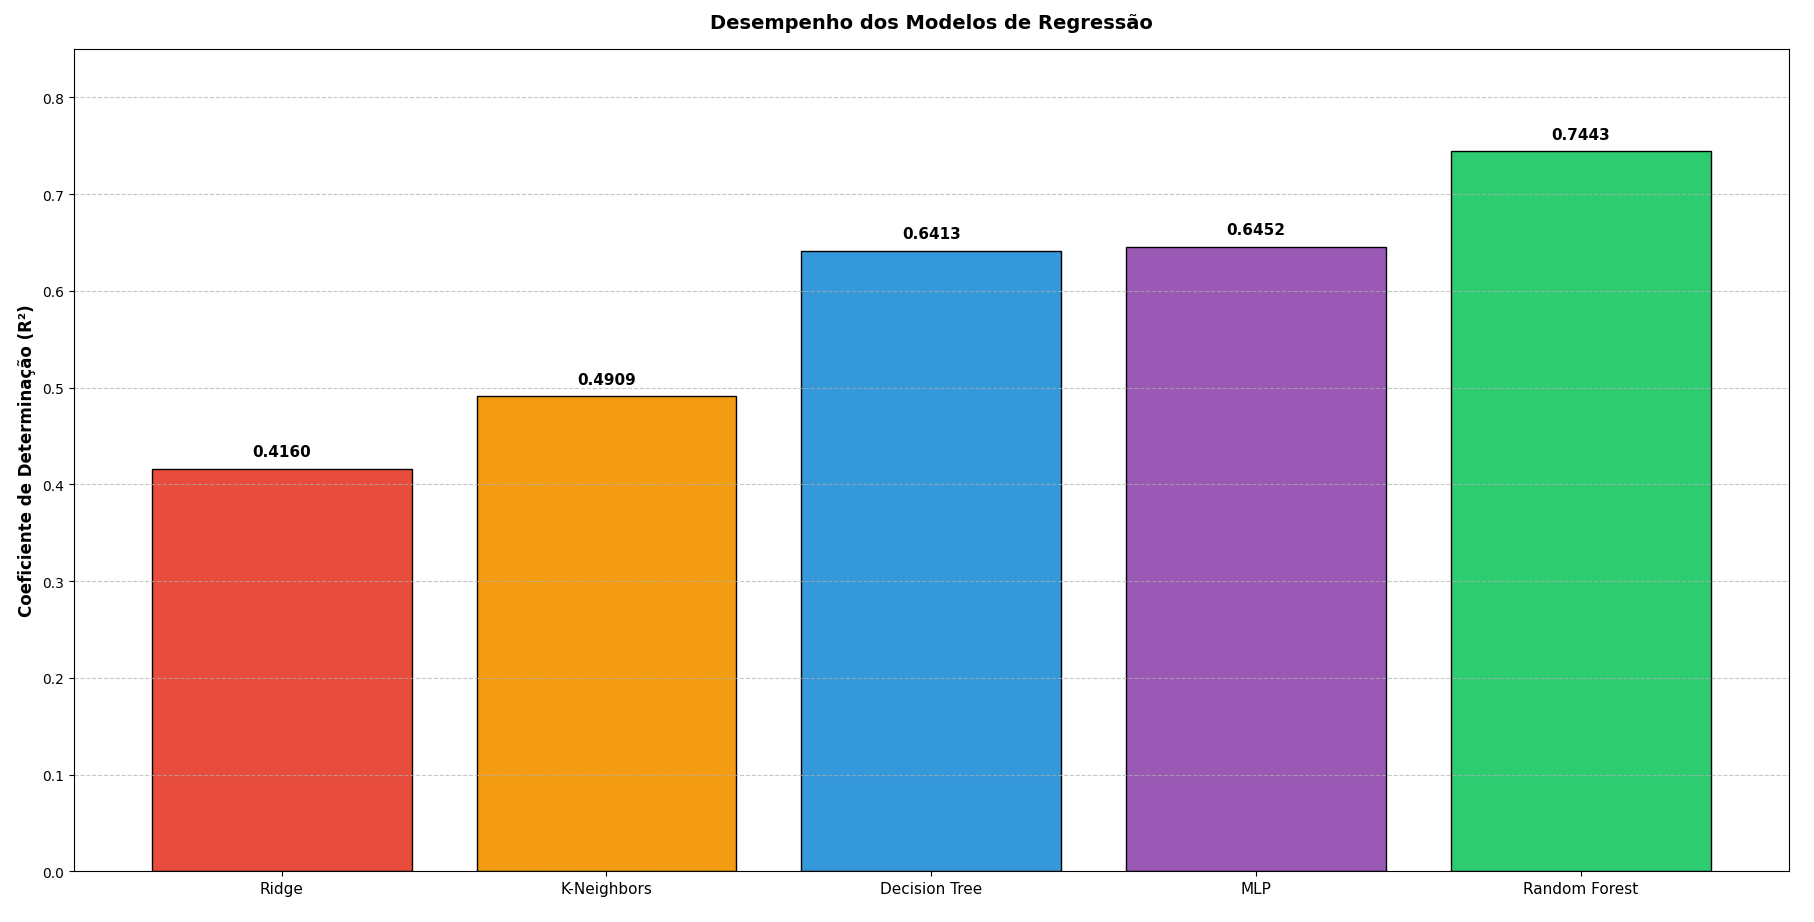
\includegraphics[width=1\linewidth]{img/grafico_r2.png}
			\caption{Comparação do Coeficiente de Determinação ($R^2$)}
			\label{fig:grafico}
		\end{figure}

		Para estabelecer a qualidade minimamente esperada (baseline) desta base de dados, considerou-se o desempenho da Regressão Ridge, um modelo linear simples. O $R^2$ de 0.416 obtido por este modelo define o limiar mínimo de aceitação, qualquer modelo preditivo para este mercado automotivo deve superar a marca de 41\% de variância explicada para justificar sua complexidade. Conforme ilustrado na Fig. \ref{fig:grafico}, o K-Neighbors obteve resultados marginalmente melhores, mas esbarrou no problema da alta dimensionalidade gerada pelas colunas binárias, que distorcem o cálculo da distância entre os veículos.

		Por outro lado, o modelo Decision Tree apresentou um grande salto de precisão ($R^2$ de 0.64). O sucesso das árvores justifica-se pela sua capacidade de criar ramificações condicionais complexas (isolando, por exemplo, veículos a diesel, automáticos e de anos recentes em "nós" específicos de alto valor). Por fim, a Random Forest obteve o melhor resultado dentre os metodos testados, visto as caracteriscas das arvores de criar condicionais complexas, se mostrando melhor que a MLP, sendo isto justificado pela grande quantidade de caracteristicas binárias na base que impoe a necessidade de se ter muito mais dados do que o disponível para o treinamento para poder se ajustar as caracteristicas.

	\section{Conclusão}

		O presente trabalho atingiu seu objetivo ao implementar e comparar um conjunto diversificado de modelos de Machine Learning para a previsão de valores de automóveis. O estudo demonstrou que o pré-processamento de dados — especialmente a remoção de outliers, o agrupamento de categorias e o tratamento de valores nulos — é tão vital para o sucesso preditivo quanto a escolha do algoritmo em si. Conclui-se que algoritmos baseados em agrupamentos não-lineares e múltiplos estimadores superam significativamente métodos estatísticos lineares em bases de dados automotivas compostas por características mistas (categóricas e contínuas).

	\begin{thebibliography}{00}
		\bibitem{r2-wikipedia} Coeficiente de determinação. Wikipédia, 2025. Disponível em: \url{https://pt.wikipedia.org/wiki/Coeficiente_de_determina%A7%C3%A3o}. Acesso em: 13 de junho de 2026.

		\bibitem{carros.com} Carros a venda. Carros.com, 2026. Disponível em: \url{https://carros.com/cars-for-sale/utah-co240/}. Acesso em: 13 de junho de 2026.
		
		\bibitem{metricas-medium} MAE, MSE, RMSE, Coefficient of Determination, Adjusted R Squared — Which Metric is Better?. Medium, 2020. Disponível em: \url{https://medium.com/analytics-vidhya/mae-mse-rmse-coefficient-of-determination-adjusted-r-squared-which-metric-is-better-cd0326a5697e}. Acesso em: 12 de junho de 2026.

		\bibitem{modelos-supervisionados} Supervised learning. Scikit-Learn. Disponível em: \url{https://scikit-learn.org/stable/supervised_learning.html}. Acesso em: 12 de junho de 2026.

		\bibitem{pandas} User Guide. Pandas. Disponível em: \url{https://pandas.pydata.org/docs/user_guide/index.html#user-guide}. Acesso em 12 de junho de 2026.

		\bibitem{matplotlib} Basic usage. Matplotlib. Disponível em: \url{https://matplotlib.org/3.5.1/tutorials/introductory/usage.html}. Acesso em: 12 de junho de 2026.

		\bibitem{stackoverflow} Como alterar CSV em Python e Pandas?. Stack Overflow, 2019. Disponível em: \url{https://pt.stackoverflow.com/questions/362420/como-alterar-csv-em-python-e-pandas}. Acesso em: 12 de junho de 2026.

		\bibitem{material-aula} Material de aula do curso de Sistemas Inteligentes, ministrado pelo professor Dr. Pablo Andretta Jaskoviak.
	\end{thebibliography}

\end{document}